% Salvare come: thesis_figures/cap3/compliance_by_design.tex
% O generare PDF con standalone e includere come compliance_by_design.pdf
\documentclass[tikz,border=10pt]{standalone}
\usepackage{tikz}
\usetikzlibrary{shapes.geometric,shapes.symbols,arrows,positioning}

\begin{document}
% \begin{figure}[htbp]
% \centering
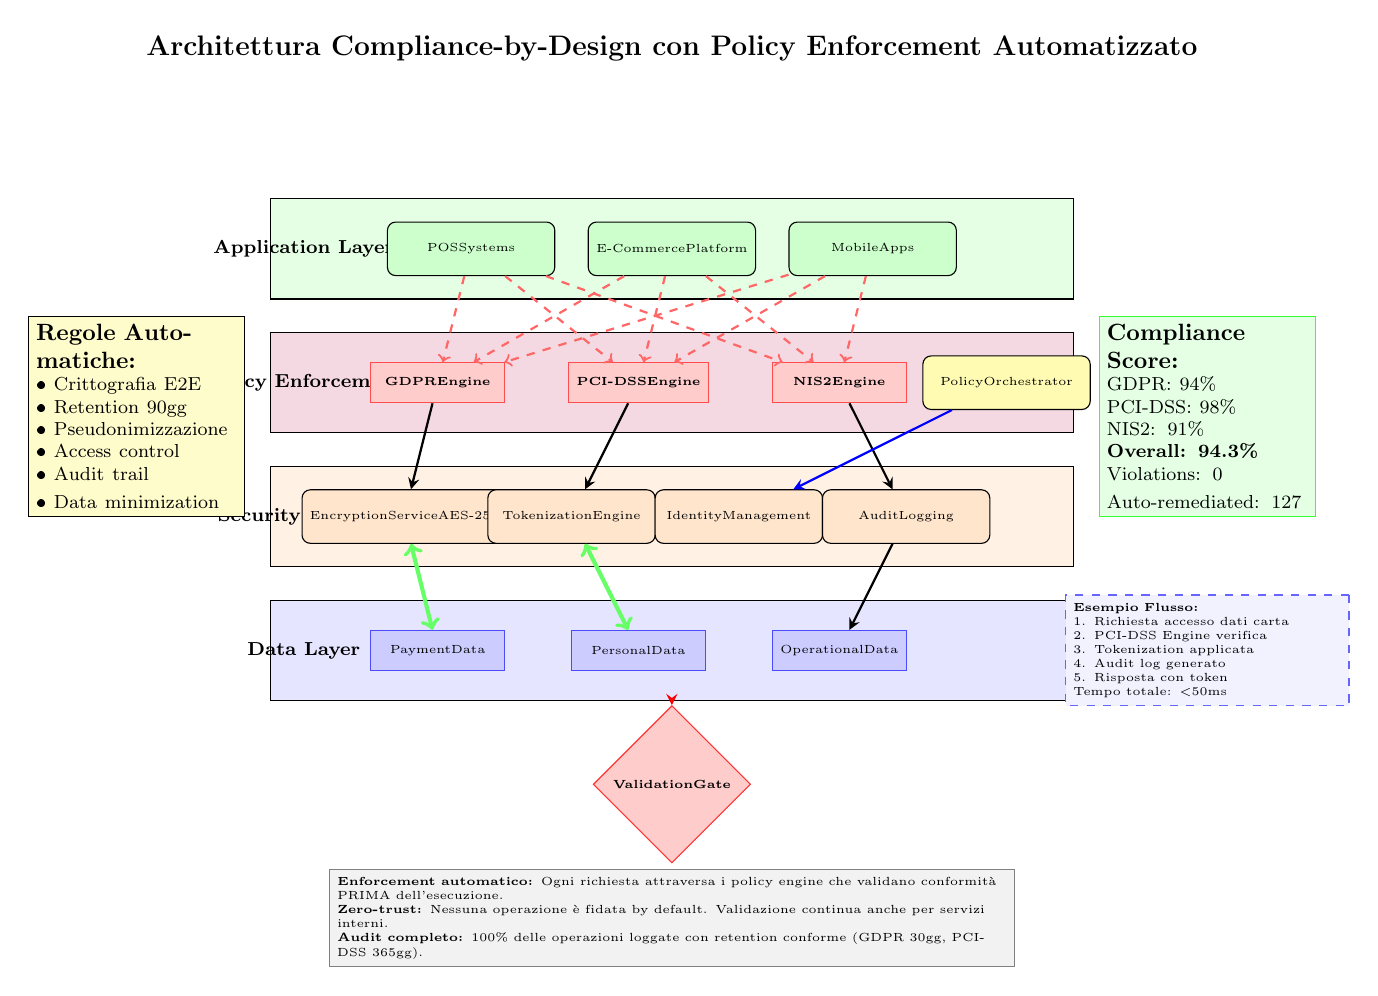
\begin{tikzpicture}[
    scale=0.85,
    transform shape,
    % Stili
    layer/.style={
        rectangle, draw, minimum width=12cm, 
        minimum height=1.5cm, font=\footnotesize
    },
    component/.style={
        rectangle, draw, rounded corners=3pt,
        minimum width=2.5cm, minimum height=0.8cm,
        font=\tiny
    },
    policy/.style={
        rectangle, draw=red!70, fill=red!20,
        minimum width=2cm, minimum height=0.6cm,
        font=\tiny\bfseries
    },
    data/.style={
        rectangle, draw=blue!70, fill=blue!20,
        minimum width=2cm, minimum height=0.6cm,
        font=\tiny
    },
    arrow/.style={->, thick, >=stealth},
    enforce/.style={->, thick, red!60, dashed},
    encrypt/.style={<->, thick, green!60, line width=1.5pt}
]

% Titolo
\node[font=\large\bfseries] at (0,9) {Architettura Compliance-by-Design con Policy Enforcement Automatizzato};

% Layer 1: Application Layer
\node[layer, fill=green!10] (app_layer) at (0,6) {};
\node[font=\footnotesize\bfseries] at (-5.5,6) {Application Layer};

\node[component, fill=green!20] (pos) at (-3,6) {POS\\Systems};
\node[component, fill=green!20] (ecom) at (0,6) {E-Commerce\\Platform};
\node[component, fill=green!20] (mobile) at (3,6) {Mobile\\Apps};

% Layer 2: Policy Enforcement Layer
\node[layer, fill=purple!15] (policy_layer) at (0,4) {};
\node[font=\footnotesize\bfseries] at (-5.5,4) {Policy Enforcement};

\node[policy] (gdpr_engine) at (-3.5,4) {GDPR\\Engine};
\node[policy] (pci_engine) at (-0.5,4) {PCI-DSS\\Engine};
\node[policy] (nis2_engine) at (2.5,4) {NIS2\\Engine};
\node[component, fill=yellow!30] (orchestrator) at (5,4) {Policy\\Orchestrator};

% Layer 3: Security Services Layer
\node[layer, fill=orange!10] (security_layer) at (0,2) {};
\node[font=\footnotesize\bfseries] at (-5.5,2) {Security Services};

\node[component, fill=orange!20] (encryption) at (-4,2) {Encryption\\Service\\AES-256};
\node[component, fill=orange!20] (tokenization) at (-1.5,2) {Tokenization\\Engine};
\node[component, fill=orange!20] (iam) at (1,2) {Identity\\Management};
\node[component, fill=orange!20] (audit) at (3.5,2) {Audit\\Logging};

% Layer 4: Data Layer
\node[layer, fill=blue!10] (data_layer) at (0,0) {};
\node[font=\footnotesize\bfseries] at (-5.5,0) {Data Layer};

\node[data] (payment) at (-3.5,0) {Payment\\Data};
\node[data] (personal) at (-0.5,0) {Personal\\Data};
\node[data] (operational) at (2.5,0) {Operational\\Data};

% Compliance Rules Box (sinistra)
\node[rectangle, draw=black, fill=yellow!20, 
      text width=3cm, align=left] at (-8,3.5) {
    \textbf{Regole Automatiche:}\\
    \footnotesize
    • Crittografia E2E\\
    • Retention 90gg\\
    • Pseudonimizzazione\\
    • Access control\\
    • Audit trail\\
    • Data minimization
};

% Metriche Compliance (destra)
\node[rectangle, draw=green!80, fill=green!10, 
      text width=3cm, align=left] at (8,3.5) {
    \textbf{Compliance Score:}\\
    \footnotesize
    GDPR: 94\%\\
    PCI-DSS: 98\%\\
    NIS2: 91\%\\
    \textbf{Overall: 94.3\%}\\
    Violations: 0\\
    Auto-remediated: 127
};

% Enforcement Flows
\foreach \app in {pos,ecom,mobile} {
    \foreach \policy in {gdpr_engine,pci_engine,nis2_engine} {
        \draw[enforce] (\app) -- (\policy);
    }
}

% Policy to Security Services
\draw[arrow, thick] (gdpr_engine) -- (encryption);
\draw[arrow, thick] (pci_engine) -- (tokenization);
\draw[arrow, thick] (nis2_engine) -- (audit);
\draw[arrow, thick, blue] (orchestrator) -- (iam);

% Security to Data
\draw[encrypt] (encryption) -- (payment);
\draw[encrypt] (tokenization) -- (personal);
\draw[arrow] (audit) -- (operational);

% Validation Checkpoint
\node[diamond, draw=red!80, fill=red!20, 
      minimum width=1.5cm, minimum height=1.5cm,
      font=\tiny\bfseries] (checkpoint) at (0,-2) {
    Validation\\Gate
};

\draw[arrow, thick, red] (data_layer) -- (checkpoint);

% Bottom info box
\node[rectangle, draw=gray, fill=gray!10, 
      text width=10cm, align=left, font=\tiny] at (0,-4) {
    \textbf{Enforcement automatico:} Ogni richiesta attraversa i policy engine che validano conformità PRIMA dell'esecuzione.\\
    \textbf{Zero-trust:} Nessuna operazione è fidata by default. Validazione continua anche per servizi interni.\\
    \textbf{Audit completo:} 100\% delle operazioni loggate con retention conforme (GDPR 30gg, PCI-DSS 365gg).
};

% Flusso esempio (box laterale)
\node[rectangle, draw=blue!60, fill=blue!5, dashed,
      text width=4cm, align=left, font=\tiny] at (8,0) {
    \textbf{Esempio Flusso:}\\
    1. Richiesta accesso dati carta\\
    2. PCI-DSS Engine verifica\\
    3. Tokenization applicata\\
    4. Audit log generato\\
    5. Risposta con token\\
    Tempo totale: <50ms
};

\end{tikzpicture}
% \caption{Architettura Compliance-by-Design con enforcement automatizzato dei requisiti normativi a livello di infrastruttura. I policy engine (GDPR, PCI-DSS, NIS2) validano ogni operazione prima dell'esecuzione, garantendo conformità by-default. Il sistema ha auto-rimediato 127 violazioni potenziali nell'ultimo mese con zero intervento manuale.}
% \label{fig:compliance_pattern}
% \end{figure}
\end{document}
#